\documentclass{article}
\usepackage{tikz}
\begin{document}
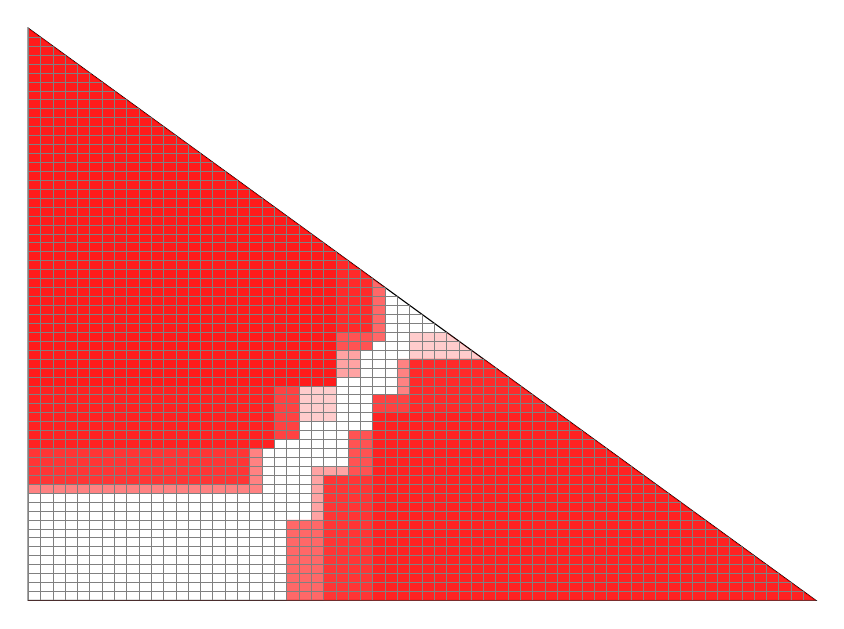
\begin{tikzpicture}[scale=10]
    \draw[clip] (0,0.7265625) |- (1,0) --cycle;
    % domains
\fill[red,fill opacity=0.2] (0.0, 0.13623046875)--(0.296875, 0.13623046875)--(0.296875, 0.1929931640625)--(0.3125, 0.1929931640625)--(0.3125, 0.204345703125)--(0.34375, 0.204345703125)--(0.34375, 0.22705078125)--(0.390625, 0.22705078125)--(0.390625, 0.2838134765625)--(0.421875, 0.2838134765625)--(0.421875, 0.31787109375)--(0.4375, 0.31787109375)--(0.4375, 0.3292236328125)--(0.453125, 0.3292236328125)--(0.453125, 0.3973388671875)--(0, 0.7265625) --cycle;
\fill[red,fill opacity=0.2] (0.0, 0.0)--(0.328125, 0.0)--(0.328125, 0.1021728515625)--(0.359375, 0.1021728515625)--(0.359375, 0.1702880859375)--(0.40625, 0.1702880859375)--(0.40625, 0.2156982421875)--(0.4375, 0.2156982421875)--(0.4375, 0.2611083984375)--(0.46875, 0.2611083984375)--(0.46875, 0.3065185546875)--(0.484375, 0.3065185546875)--(0.484375, 0.340576171875)--(0.53125, 0.340576171875)--(1, 0)--(0, 0) -- cycle;
\fill[red,fill opacity=0.2] (0.0, 0.13623046875)--(0.296875, 0.13623046875)--(0.296875, 0.1929931640625)--(0.3125, 0.1929931640625)--(0.3125, 0.204345703125)--(0.34375, 0.204345703125)--(0.34375, 0.2724609375)--(0.390625, 0.2724609375)--(0.390625, 0.2838134765625)--(0.421875, 0.2838134765625)--(0.421875, 0.31787109375)--(0.4375, 0.31787109375)--(0.4375, 0.3292236328125)--(0.453125, 0.3292236328125)--(0.453125, 0.3973388671875)--(0, 0.7265625) --cycle;
\fill[red,fill opacity=0.2] (0.0, 0.0)--(0.328125, 0.0)--(0.328125, 0.1021728515625)--(0.359375, 0.1021728515625)--(0.359375, 0.1702880859375)--(0.40625, 0.1702880859375)--(0.40625, 0.2156982421875)--(0.4375, 0.2156982421875)--(0.4375, 0.2611083984375)--(0.46875, 0.2611083984375)--(0.46875, 0.3065185546875)--(0.578125, 0.3065185546875)--(1, 0)--(0, 0) -- cycle;
\fill[red,fill opacity=0.2] (0.0, 0.13623046875)--(0.296875, 0.13623046875)--(0.296875, 0.1929931640625)--(0.3125, 0.1929931640625)--(0.3125, 0.204345703125)--(0.34375, 0.204345703125)--(0.34375, 0.2724609375)--(0.390625, 0.2724609375)--(0.390625, 0.31787109375)--(0.4375, 0.31787109375)--(0.4375, 0.3292236328125)--(0.453125, 0.3292236328125)--(0.453125, 0.3973388671875)--(0, 0.7265625) --cycle;
\fill[red,fill opacity=0.2] (0.0, 0.0)--(0.328125, 0.0)--(0.328125, 0.1021728515625)--(0.375, 0.1021728515625)--(0.375, 0.158935546875)--(0.40625, 0.158935546875)--(0.40625, 0.2156982421875)--(0.4375, 0.2156982421875)--(0.4375, 0.2611083984375)--(0.46875, 0.2611083984375)--(0.46875, 0.3065185546875)--(0.578125, 0.3065185546875)--(1, 0)--(0, 0) -- cycle;
\fill[red,fill opacity=0.2] (0.0, 0.1475830078125)--(0.28125, 0.1475830078125)--(0.28125, 0.1929931640625)--(0.3125, 0.1929931640625)--(0.3125, 0.204345703125)--(0.34375, 0.204345703125)--(0.34375, 0.2724609375)--(0.390625, 0.2724609375)--(0.390625, 0.31787109375)--(0.4375, 0.31787109375)--(0.4375, 0.3292236328125)--(0.453125, 0.3292236328125)--(0.453125, 0.3973388671875)--(0, 0.7265625) --cycle;
\fill[red,fill opacity=0.2] (0.0, 0.0)--(0.328125, 0.0)--(0.328125, 0.1021728515625)--(0.375, 0.1021728515625)--(0.375, 0.158935546875)--(0.40625, 0.158935546875)--(0.40625, 0.2156982421875)--(0.4375, 0.2156982421875)--(0.4375, 0.2611083984375)--(0.484375, 0.2611083984375)--(0.484375, 0.3065185546875)--(0.578125, 0.3065185546875)--(1, 0)--(0, 0) -- cycle;
\fill[red,fill opacity=0.2] (0.0, 0.1475830078125)--(0.28125, 0.1475830078125)--(0.28125, 0.1929931640625)--(0.3125, 0.1929931640625)--(0.3125, 0.204345703125)--(0.34375, 0.204345703125)--(0.34375, 0.2724609375)--(0.390625, 0.2724609375)--(0.390625, 0.31787109375)--(0.4375, 0.31787109375)--(0.4375, 0.40869140625)--(0, 0.7265625) --cycle;
\fill[red,fill opacity=0.2] (0.0, 0.0)--(0.375, 0.0)--(0.375, 0.158935546875)--(0.40625, 0.158935546875)--(0.40625, 0.2156982421875)--(0.4375, 0.2156982421875)--(0.4375, 0.2611083984375)--(0.484375, 0.2611083984375)--(0.484375, 0.3065185546875)--(0.578125, 0.3065185546875)--(1, 0)--(0, 0) -- cycle;
\fill[red,fill opacity=0.2] (0.0, 0.1475830078125)--(0.28125, 0.1475830078125)--(0.28125, 0.1929931640625)--(0.3125, 0.1929931640625)--(0.3125, 0.204345703125)--(0.34375, 0.204345703125)--(0.34375, 0.2724609375)--(0.390625, 0.2724609375)--(0.390625, 0.340576171875)--(0.4375, 0.340576171875)--(0.4375, 0.40869140625)--(0, 0.7265625) --cycle;
\fill[red,fill opacity=0.2] (0.0, 0.0)--(0.375, 0.0)--(0.375, 0.158935546875)--(0.4375, 0.158935546875)--(0.4375, 0.2611083984375)--(0.484375, 0.2611083984375)--(0.484375, 0.3065185546875)--(0.578125, 0.3065185546875)--(1, 0)--(0, 0) -- cycle;
\fill[red,fill opacity=0.2] (0.0, 0.1475830078125)--(0.28125, 0.1475830078125)--(0.28125, 0.1929931640625)--(0.3125, 0.1929931640625)--(0.3125, 0.2724609375)--(0.390625, 0.2724609375)--(0.390625, 0.340576171875)--(0.4375, 0.340576171875)--(0.4375, 0.40869140625)--(0, 0.7265625) --cycle;
\fill[red,fill opacity=0.2] (0.0, 0.0)--(0.375, 0.0)--(0.375, 0.158935546875)--(0.4375, 0.158935546875)--(0.4375, 0.2384033203125)--(0.484375, 0.2384033203125)--(0.484375, 0.3065185546875)--(0.578125, 0.3065185546875)--(1, 0)--(0, 0) -- cycle;
\fill[red,fill opacity=0.2] (0.0, 0.1929931640625)--(0.3125, 0.1929931640625)--(0.3125, 0.2724609375)--(0.390625, 0.2724609375)--(0.390625, 0.340576171875)--(0.4375, 0.340576171875)--(0.4375, 0.40869140625)--(0, 0.7265625) --cycle;
\fill[red,fill opacity=0.2] (0.0, 0.0)--(0.4375, 0.0)--(0.4375, 0.2384033203125)--(0.484375, 0.2384033203125)--(0.484375, 0.3065185546875)--(0.578125, 0.3065185546875)--(1, 0)--(0, 0) -- cycle;
\fill[red,fill opacity=0.2] (0.0, 0.1929931640625)--(0.3125, 0.1929931640625)--(0.3125, 0.2724609375)--(0.390625, 0.2724609375)--(0.390625, 0.4427490234375)--(0, 0.7265625) --cycle;
\fill[red,fill opacity=0.2] (0.0, 0.0)--(0.4375, 0.0)--(0.4375, 0.2384033203125)--(0.671875, 0.2384033203125)--(1, 0)--(0, 0) -- cycle;
\fill[red,fill opacity=0.2] (0.0, 0.2724609375)--(0.390625, 0.2724609375)--(0.390625, 0.4427490234375)--(0, 0.7265625) --cycle;
    \draw[help lines,yscale=0.7265625] (0,0) grid[step=0.015625] (1,1);
\end{tikzpicture}


We found the excluded regions shown above.

\newpage
The complement of the upper
excluded region (picture below) has the smallest eigenvalue above the
threshold 12.25. Yet it must contain the nodal domain which has eigenvalue
below that threshold. This gives a contradiction with the domain
monotonicity.

Vertices:

[(0, 12), (19, 12), (19, 17), (20, 17), (20, 18), (22, 18), (22, 20), (25, 20), (25, 25), (27, 25), (27, 28), (28, 28), (28, 29), (29, 29), (29, 35), [(64, 0), (0, 0)]]

Unprocessed eigenvalues:

[2.1633503059163846, 11.02534301446005]

Residuals:

[4.598151070361678e-12, 6.9581514886418879e-12]

Rescaled eigenvalues (but not postprocessed):

[  2.16335031  11.02534301]

Postprocessed eigenvalue (lower bound):

12.2833697245

    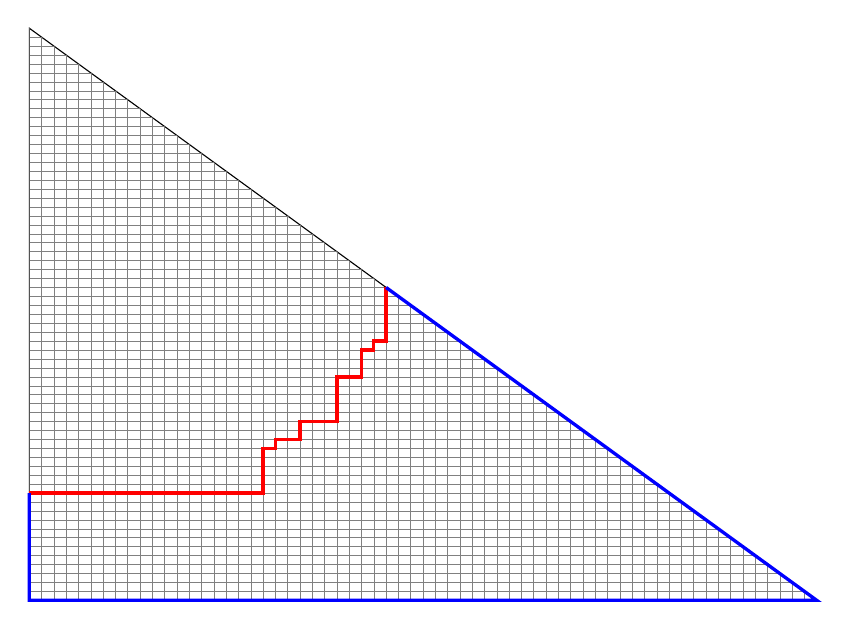
\begin{tikzpicture}[scale=10]
    \begin{scope}
    \draw[clip] (0,0.7265625) |- (1,0) --cycle;
    \draw[help lines,yscale=0.7265625] (0,0) grid[step=0.015625] (1,1);
    \end{scope}
    \draw[very thick, red](0.0, 0.13623046875)--(0.296875, 0.13623046875)--(0.296875, 0.1929931640625)--(0.3125, 0.1929931640625)--(0.3125, 0.204345703125)--(0.34375, 0.204345703125)--(0.34375, 0.22705078125)--(0.390625, 0.22705078125)--(0.390625, 0.2838134765625)--(0.421875, 0.2838134765625)--(0.421875, 0.31787109375)--(0.4375, 0.31787109375)--(0.4375, 0.3292236328125)--(0.453125, 0.3292236328125)--(0.453125, 0.3973388671875)coordinate (a); \draw[very thick,blue] (a) -- (1,0) -- (0,0) -- (0.0, 0.13623046875);
\end{tikzpicture}\begin{enumerate}
\newpage
\item New vertex $p$ in upper excluded region $U^{1}$:
(25, 24) (in grid coordinates).

Vertices of the upper domain $D_U(p)$:

[(0, 0), (25, 0), (25, 24), (40, 24), [(0, 64)]]

Unprocessed eigenvalues for the upper domain:

[2.1693043007060915, 10.783508211644577]

Residuals:

[5.195405372448488e-12, 6.945071811605383e-12]

Rescaled eigenvalues (by the bottom side length), but not postprocessed:

[ 12.32808937  61.28234427]

Postprocesses eigenvalue (lower bound):

12.3171461311

Eigenvalue for lower test domain $D_L^{test}$: 10.1477943063 (does not need to
be calculated until it reaches the threshold 12.25).

    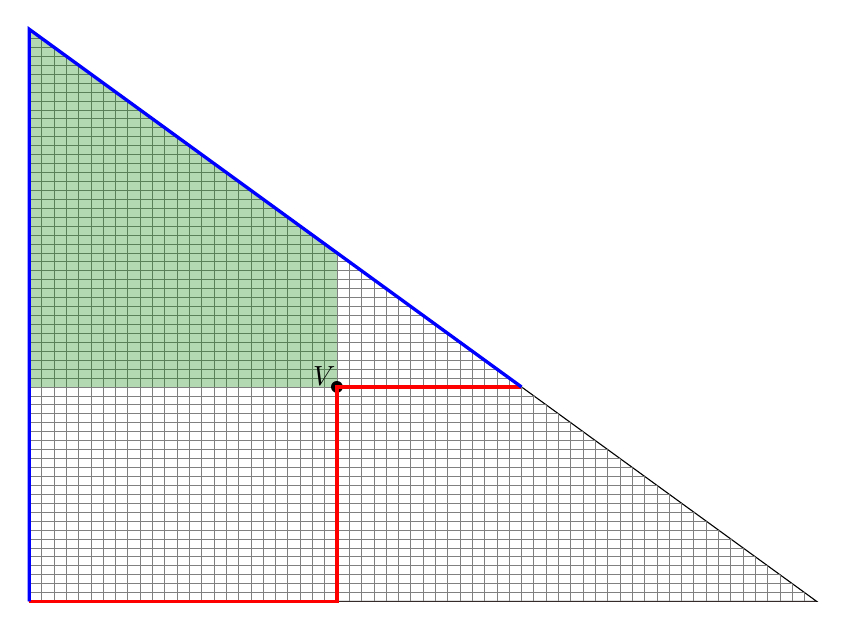
\begin{tikzpicture}[scale=10]
    \begin{scope}
    \draw[clip] (0,0.7265625) |- (1,0) --cycle;
    \draw[help lines,yscale=0.7265625] (0,0) grid[step=0.015625] (1,1);
    \fill[red,fill opacity=0.3] (0.0, 0.0)--(1.0, 0.0)--(1, 0)--(0, 0) -- cycle;
\fill[magenta,fill opacity=0.3] (0.0, 0.0)--(0.0, 0.7265625)--(0, 0.7265625) -- cycle;

    \fill[green!50!black,opacity=0.3] (0,0.7265625) rectangle (0.390625, 0.2724609375) node
    [shape=circle,fill=black,fill opacity=1,minimum size=1.5mm,inner sep=0pt,
    outer sep=0pt] {} node [above left=-3pt,black,opacity=1]
     { $V$};\end{scope}\draw[very thick, red](0.0, 0.0)--(0.390625, 0.0)--(0.390625, 0.2724609375)--(0.625, 0.2724609375)coordinate (a);
\draw[very thick, blue] (a) -- (0,0.7265625) -- (0,0);
\end{tikzpicture}

\newpage
\item New vertex $p$ in lower excluded region $L^{1}$:
(28, 21) (in grid coordinates).

Vertices for the lower domain $D_L(p)$:

[(0, 21), (28, 21), (28, 36), [(64, 0), (0, 0)]]

Unprocessed eigenvalues for the lower domain:

[2.1746523460623877, 8.3827823956042327]

Residuals:

[4.913715035163391e-12, 7.6916267788076862e-12]

Rescaled eigenvalues (by bottom side length), but not postprocessed:

[ 12.35848215  47.63909357]

Postprocesses eigenvalue (lower bound):

12.347484908

Eigenvalue for upper test domain $D_U^{test}$: 10.9964075789 (does not need to
be calculated until it reaches the threshold 12.25).

    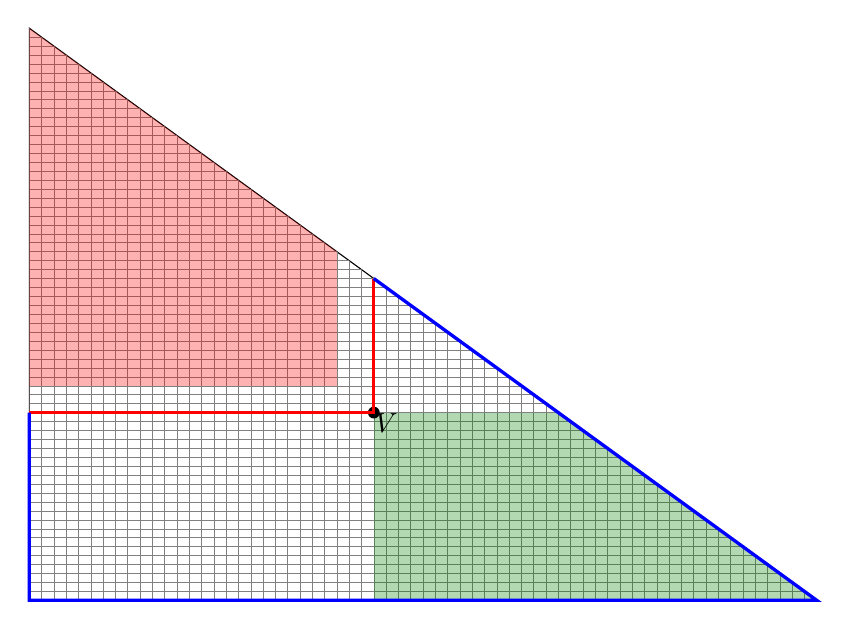
\begin{tikzpicture}[scale=10]
    \begin{scope}
    \draw[clip] (0,0.7265625) |- (1,0) --cycle;
    \draw[help lines,yscale=0.7265625] (0,0) grid[step=0.015625] (1,1);
    \fill[red,fill opacity=0.3] (0.0, 0.0)--(0.0, 0.2724609375)--(0.390625, 0.2724609375)--(0.390625, 0.4427490234375)--(0, 0.7265625) -- cycle;
\fill[magenta,fill opacity=0.3] (0.0, 0.0)--(1.0, 0.0)--(1, 0)--(0, 0) -- cycle;

    \fill[green!50!black,opacity=0.3] (1,0) rectangle (0.4375, 0.2384033203125) node
    [shape=circle,fill=black,fill opacity=1,minimum size=1.5mm,
    inner sep=0pt,outer sep=0pt] {} node [below right=-3pt,black,opacity=1]
     { $V$};\end{scope}\draw[very thick, red](0.0, 0.2384033203125)--(0.4375, 0.2384033203125)--(0.4375, 0.40869140625)coordinate (a);
\draw[very thick, blue] (a) -- (1,0) -- (0,0) -- (0.0, 0.2384033203125);
\end{tikzpicture}

\newpage
\item New vertex $p$ in upper excluded region $U^{2}$:
(20, 17) (in grid coordinates).

Vertices of the upper domain $D_U(p)$:

[(0, 0), (20, 0), (20, 17), (28, 17), (28, 21), (43, 21), [(0, 64)]]

Unprocessed eigenvalues for the upper domain:

[2.1609297493267277, 11.105649612004703]

Residuals:

[4.8723116845836387e-12, 7.4090307603537676e-12]

Rescaled eigenvalues (by the bottom side length), but not postprocessed:

[ 12.28049706  63.11306391]

Postprocesses eigenvalue (lower bound):

12.2696381062

Eigenvalue for lower test domain $D_L^{test}$: 10.8384636507 (does not need to
be calculated until it reaches the threshold 12.25).

    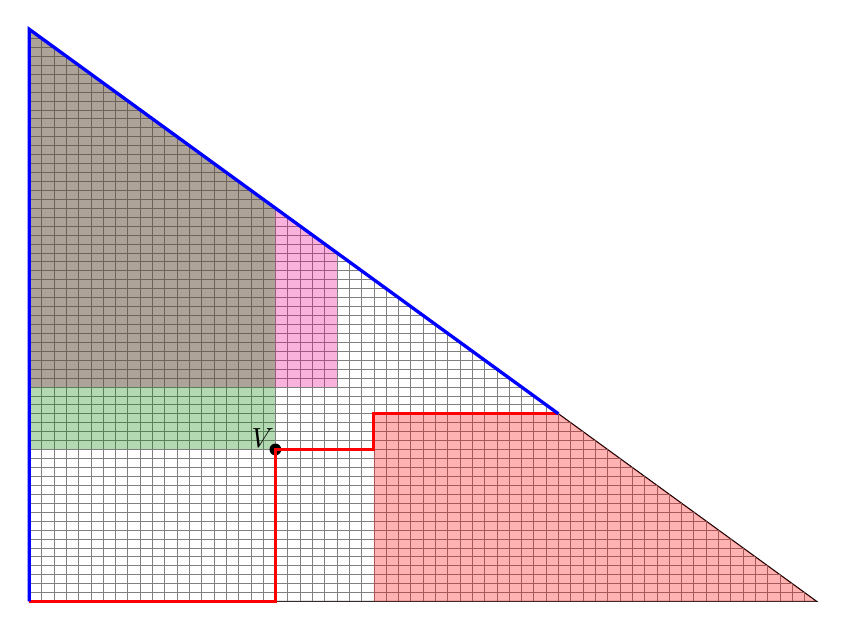
\begin{tikzpicture}[scale=10]
    \begin{scope}
    \draw[clip] (0,0.7265625) |- (1,0) --cycle;
    \draw[help lines,yscale=0.7265625] (0,0) grid[step=0.015625] (1,1);
    \fill[red,fill opacity=0.3] (0.0, 0.0)--(0.4375, 0.0)--(0.4375, 0.2384033203125)--(0.671875, 0.2384033203125)--(1, 0)--(0, 0) -- cycle;
\fill[magenta,fill opacity=0.3] (0.0, 0.0)--(0.0, 0.2724609375)--(0.390625, 0.2724609375)--(0.390625, 0.4427490234375)--(0, 0.7265625) -- cycle;

    \fill[green!50!black,opacity=0.3] (0,0.7265625) rectangle (0.3125, 0.1929931640625) node
    [shape=circle,fill=black,fill opacity=1,minimum size=1.5mm,inner sep=0pt,
    outer sep=0pt] {} node [above left=-3pt,black,opacity=1]
     { $V$};\end{scope}\draw[very thick, red](0.0, 0.0)--(0.3125, 0.0)--(0.3125, 0.1929931640625)--(0.4375, 0.1929931640625)--(0.4375, 0.2384033203125)--(0.671875, 0.2384033203125)coordinate (a);
\draw[very thick, blue] (a) -- (0,0.7265625) -- (0,0);
\end{tikzpicture}

\newpage
\item New vertex $p$ in lower excluded region $L^{2}$:
(31, 27) (in grid coordinates).

Vertices for the lower domain $D_L(p)$:

[(0, 17), (20, 17), (20, 24), (25, 24), (25, 27), (31, 27), (31, 33), [(64, 0), (0, 0)]]

Unprocessed eigenvalues for the lower domain:

[2.1607701681727698, 9.8954267447091855]

Residuals:

[4.5639143759865585e-12, 7.942461693353896e-12]

Rescaled eigenvalues (by bottom side length), but not postprocessed:

[ 12.27959016  56.23540471]

Postprocesses eigenvalue (lower bound):

12.2687328145

Eigenvalue for upper test domain $D_U^{test}$: 11.3481893437 (does not need to
be calculated until it reaches the threshold 12.25).

    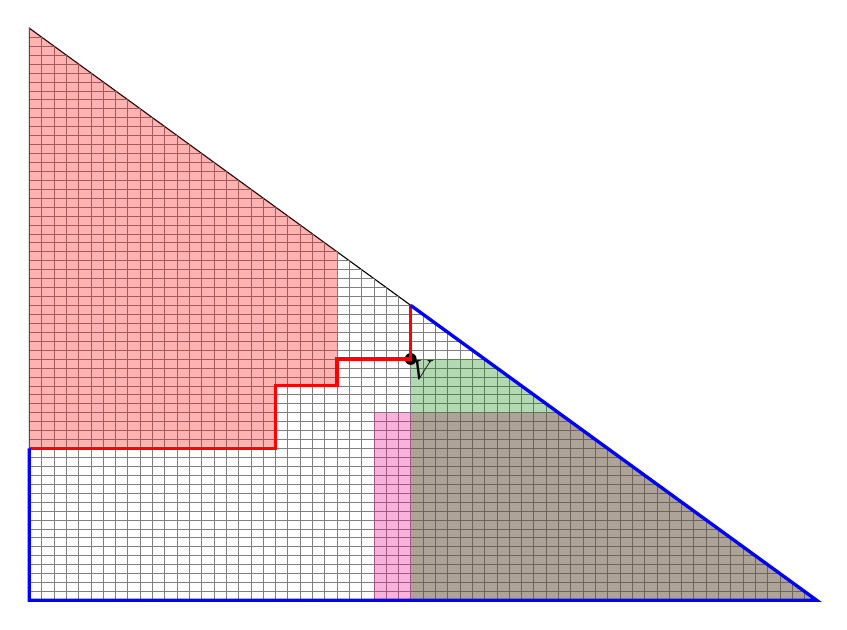
\begin{tikzpicture}[scale=10]
    \begin{scope}
    \draw[clip] (0,0.7265625) |- (1,0) --cycle;
    \draw[help lines,yscale=0.7265625] (0,0) grid[step=0.015625] (1,1);
    \fill[red,fill opacity=0.3] (0.0, 0.0)--(0.0, 0.1929931640625)--(0.3125, 0.1929931640625)--(0.3125, 0.2724609375)--(0.390625, 0.2724609375)--(0.390625, 0.4427490234375)--(0, 0.7265625) -- cycle;
\fill[magenta,fill opacity=0.3] (0.0, 0.0)--(0.4375, 0.0)--(0.4375, 0.2384033203125)--(0.671875, 0.2384033203125)--(1, 0)--(0, 0) -- cycle;

    \fill[green!50!black,opacity=0.3] (1,0) rectangle (0.484375, 0.3065185546875) node
    [shape=circle,fill=black,fill opacity=1,minimum size=1.5mm,
    inner sep=0pt,outer sep=0pt] {} node [below right=-3pt,black,opacity=1]
     { $V$};\end{scope}\draw[very thick, red](0.0, 0.1929931640625)--(0.3125, 0.1929931640625)--(0.3125, 0.2724609375)--(0.390625, 0.2724609375)--(0.390625, 0.3065185546875)--(0.484375, 0.3065185546875)--(0.484375, 0.3746337890625)coordinate (a);
\draw[very thick, blue] (a) -- (1,0) -- (0,0) -- (0.0, 0.1929931640625);
\end{tikzpicture}

\newpage
\item New vertex $p$ in upper excluded region $U^{3}$:
(28, 30) (in grid coordinates).

Vertices of the upper domain $D_U(p)$:

[(0, 0), (28, 0), (28, 30), (34, 30), [(0, 64)]]

Unprocessed eigenvalues for the upper domain:

[2.1592022649722211, 10.509175135495724]

Residuals:

[5.1257783330952429e-12, 7.9911062056934245e-12]

Rescaled eigenvalues (by the bottom side length), but not postprocessed:

[ 12.27067982  59.72331787]

Postprocesses eigenvalue (lower bound):

12.259838213

Eigenvalue for lower test domain $D_L^{test}$: 11.1543395403 (does not need to
be calculated until it reaches the threshold 12.25).

    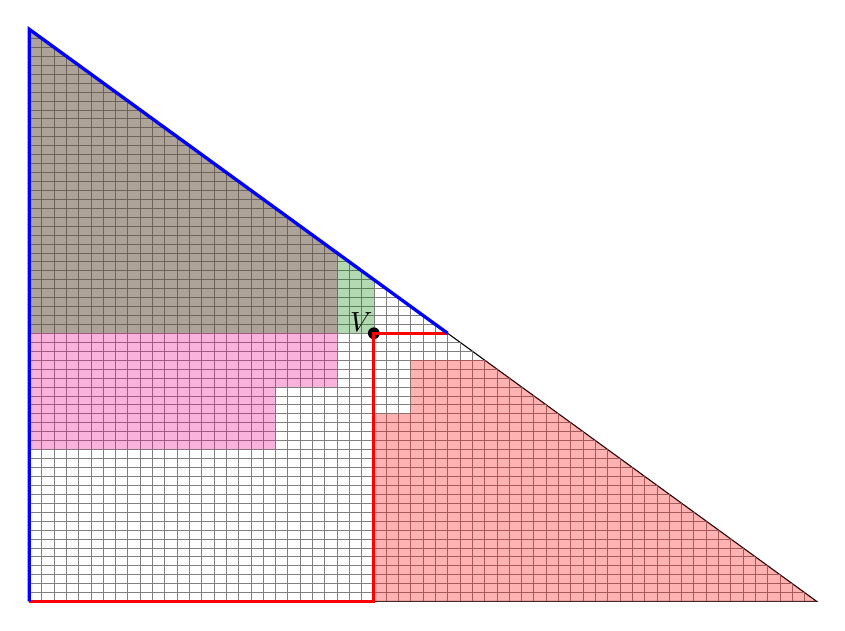
\begin{tikzpicture}[scale=10]
    \begin{scope}
    \draw[clip] (0,0.7265625) |- (1,0) --cycle;
    \draw[help lines,yscale=0.7265625] (0,0) grid[step=0.015625] (1,1);
    \fill[red,fill opacity=0.3] (0.0, 0.0)--(0.4375, 0.0)--(0.4375, 0.2384033203125)--(0.484375, 0.2384033203125)--(0.484375, 0.3065185546875)--(0.578125, 0.3065185546875)--(1, 0)--(0, 0) -- cycle;
\fill[magenta,fill opacity=0.3] (0.0, 0.0)--(0.0, 0.1929931640625)--(0.3125, 0.1929931640625)--(0.3125, 0.2724609375)--(0.390625, 0.2724609375)--(0.390625, 0.4427490234375)--(0, 0.7265625) -- cycle;

    \fill[green!50!black,opacity=0.3] (0,0.7265625) rectangle (0.4375, 0.340576171875) node
    [shape=circle,fill=black,fill opacity=1,minimum size=1.5mm,inner sep=0pt,
    outer sep=0pt] {} node [above left=-3pt,black,opacity=1]
     { $V$};\end{scope}\draw[very thick, red](0.0, 0.0)--(0.4375, 0.0)--(0.4375, 0.340576171875)--(0.53125, 0.340576171875)coordinate (a);
\draw[very thick, blue] (a) -- (0,0.7265625) -- (0,0);
\end{tikzpicture}

\newpage
\item New vertex $p$ in lower excluded region $L^{3}$:
(24, 14) (in grid coordinates).

Vertices for the lower domain $D_L(p)$:

[(0, 14), (24, 14), (24, 24), (25, 24), (25, 30), (28, 30), (28, 36), [(64, 0), (0, 0)]]

Unprocessed eigenvalues for the lower domain:

[2.1837241362172217, 11.23991415603915]

Residuals:

[4.7787436788803418e-12, 7.0826552423146707e-12]

Rescaled eigenvalues (by bottom side length), but not postprocessed:

[ 12.41003685  63.87608517]

Postprocesses eigenvalue (lower bound):

12.3989477089

Eigenvalue for upper test domain $D_U^{test}$: 11.5949767668 (does not need to
be calculated until it reaches the threshold 12.25).

    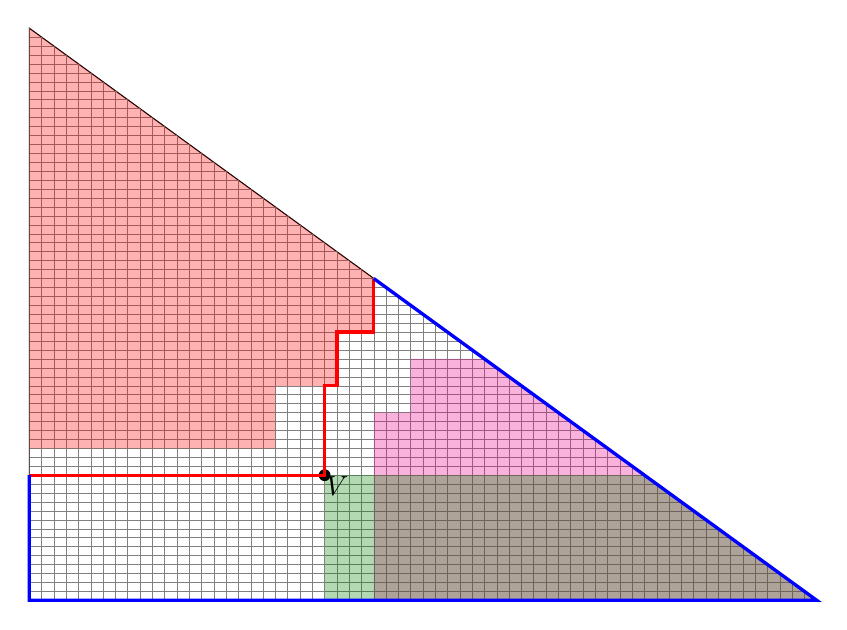
\begin{tikzpicture}[scale=10]
    \begin{scope}
    \draw[clip] (0,0.7265625) |- (1,0) --cycle;
    \draw[help lines,yscale=0.7265625] (0,0) grid[step=0.015625] (1,1);
    \fill[red,fill opacity=0.3] (0.0, 0.0)--(0.0, 0.1929931640625)--(0.3125, 0.1929931640625)--(0.3125, 0.2724609375)--(0.390625, 0.2724609375)--(0.390625, 0.340576171875)--(0.4375, 0.340576171875)--(0.4375, 0.40869140625)--(0, 0.7265625) -- cycle;
\fill[magenta,fill opacity=0.3] (0.0, 0.0)--(0.4375, 0.0)--(0.4375, 0.2384033203125)--(0.484375, 0.2384033203125)--(0.484375, 0.3065185546875)--(0.578125, 0.3065185546875)--(1, 0)--(0, 0) -- cycle;

    \fill[green!50!black,opacity=0.3] (1,0) rectangle (0.375, 0.158935546875) node
    [shape=circle,fill=black,fill opacity=1,minimum size=1.5mm,
    inner sep=0pt,outer sep=0pt] {} node [below right=-3pt,black,opacity=1]
     { $V$};\end{scope}\draw[very thick, red](0.0, 0.158935546875)--(0.375, 0.158935546875)--(0.375, 0.2724609375)--(0.390625, 0.2724609375)--(0.390625, 0.340576171875)--(0.4375, 0.340576171875)--(0.4375, 0.40869140625)coordinate (a);
\draw[very thick, blue] (a) -- (1,0) -- (0,0) -- (0.0, 0.158935546875);
\end{tikzpicture}

\newpage
\item New vertex $p$ in upper excluded region $U^{4}$:
(18, 13) (in grid coordinates).

Vertices of the upper domain $D_U(p)$:

[(0, 0), (18, 0), (18, 13), (24, 13), (24, 14), (28, 14), (28, 21), (31, 21), (31, 27), (37, 27), [(0, 64)]]

Unprocessed eigenvalues for the upper domain:

[2.1616790644024646, 11.146739955047408]

Residuals:

[4.8383576680934513e-12, 7.4096545152980828e-12]

Rescaled eigenvalues (by the bottom side length), but not postprocessed:

[ 12.28475539  63.34657906]

Postprocesses eigenvalue (lower bound):

12.2738889118

Eigenvalue for lower test domain $D_L^{test}$: 11.3641881646 (does not need to
be calculated until it reaches the threshold 12.25).

    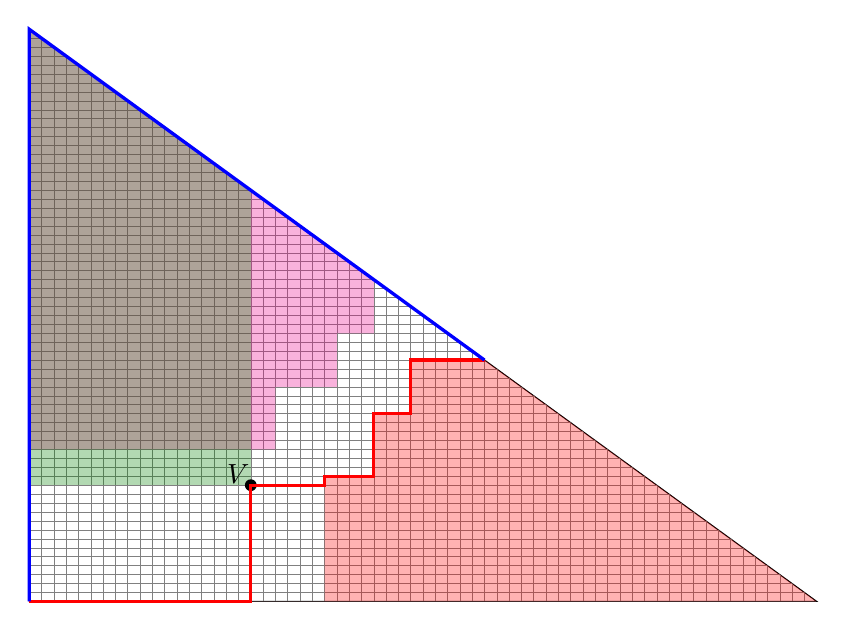
\begin{tikzpicture}[scale=10]
    \begin{scope}
    \draw[clip] (0,0.7265625) |- (1,0) --cycle;
    \draw[help lines,yscale=0.7265625] (0,0) grid[step=0.015625] (1,1);
    \fill[red,fill opacity=0.3] (0.0, 0.0)--(0.375, 0.0)--(0.375, 0.158935546875)--(0.4375, 0.158935546875)--(0.4375, 0.2384033203125)--(0.484375, 0.2384033203125)--(0.484375, 0.3065185546875)--(0.578125, 0.3065185546875)--(1, 0)--(0, 0) -- cycle;
\fill[magenta,fill opacity=0.3] (0.0, 0.0)--(0.0, 0.1929931640625)--(0.3125, 0.1929931640625)--(0.3125, 0.2724609375)--(0.390625, 0.2724609375)--(0.390625, 0.340576171875)--(0.4375, 0.340576171875)--(0.4375, 0.40869140625)--(0, 0.7265625) -- cycle;

    \fill[green!50!black,opacity=0.3] (0,0.7265625) rectangle (0.28125, 0.1475830078125) node
    [shape=circle,fill=black,fill opacity=1,minimum size=1.5mm,inner sep=0pt,
    outer sep=0pt] {} node [above left=-3pt,black,opacity=1]
     { $V$};\end{scope}\draw[very thick, red](0.0, 0.0)--(0.28125, 0.0)--(0.28125, 0.1475830078125)--(0.375, 0.1475830078125)--(0.375, 0.158935546875)--(0.4375, 0.158935546875)--(0.4375, 0.2384033203125)--(0.484375, 0.2384033203125)--(0.484375, 0.3065185546875)--(0.578125, 0.3065185546875)coordinate (a);
\draw[very thick, blue] (a) -- (0,0.7265625) -- (0,0);
\end{tikzpicture}

\newpage
\item New vertex $p$ in lower excluded region $L^{4}$:
(28, 23) (in grid coordinates).

Vertices for the lower domain $D_L(p)$:

[(0, 13), (18, 13), (18, 17), (20, 17), (20, 23), (28, 23), (28, 36), [(64, 0), (0, 0)]]

Unprocessed eigenvalues for the lower domain:

[2.1593603202112912, 10.765645575090153]

Residuals:

[4.6027322175280276e-12, 7.397046232424909e-12]

Rescaled eigenvalues (by bottom side length), but not postprocessed:

[ 12.27157804  61.18083146]

Postprocesses eigenvalue (lower bound):

12.2607348494

Eigenvalue for upper test domain $D_U^{test}$: 11.7004951476 (does not need to
be calculated until it reaches the threshold 12.25).

    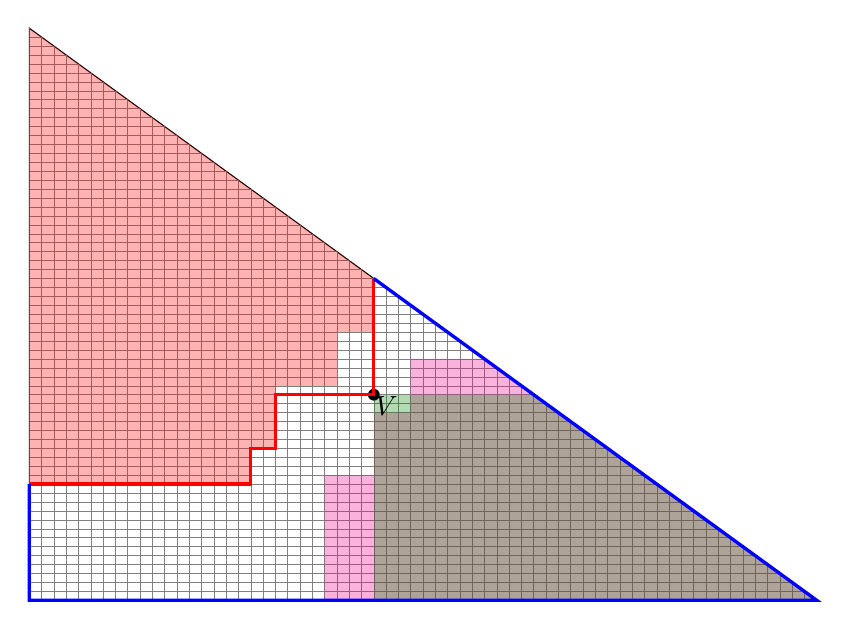
\begin{tikzpicture}[scale=10]
    \begin{scope}
    \draw[clip] (0,0.7265625) |- (1,0) --cycle;
    \draw[help lines,yscale=0.7265625] (0,0) grid[step=0.015625] (1,1);
    \fill[red,fill opacity=0.3] (0.0, 0.0)--(0.0, 0.1475830078125)--(0.28125, 0.1475830078125)--(0.28125, 0.1929931640625)--(0.3125, 0.1929931640625)--(0.3125, 0.2724609375)--(0.390625, 0.2724609375)--(0.390625, 0.340576171875)--(0.4375, 0.340576171875)--(0.4375, 0.40869140625)--(0, 0.7265625) -- cycle;
\fill[magenta,fill opacity=0.3] (0.0, 0.0)--(0.375, 0.0)--(0.375, 0.158935546875)--(0.4375, 0.158935546875)--(0.4375, 0.2384033203125)--(0.484375, 0.2384033203125)--(0.484375, 0.3065185546875)--(0.578125, 0.3065185546875)--(1, 0)--(0, 0) -- cycle;

    \fill[green!50!black,opacity=0.3] (1,0) rectangle (0.4375, 0.2611083984375) node
    [shape=circle,fill=black,fill opacity=1,minimum size=1.5mm,
    inner sep=0pt,outer sep=0pt] {} node [below right=-3pt,black,opacity=1]
     { $V$};\end{scope}\draw[very thick, red](0.0, 0.1475830078125)--(0.28125, 0.1475830078125)--(0.28125, 0.1929931640625)--(0.3125, 0.1929931640625)--(0.3125, 0.2611083984375)--(0.4375, 0.2611083984375)--(0.4375, 0.40869140625)coordinate (a);
\draw[very thick, blue] (a) -- (1,0) -- (0,0) -- (0.0, 0.1475830078125);
\end{tikzpicture}

\newpage
\item New vertex $p$ in upper excluded region $U^{5}$:
(22, 18) (in grid coordinates).

Vertices of the upper domain $D_U(p)$:

[(0, 0), (22, 0), (22, 18), (28, 18), (28, 23), (31, 23), (31, 27), (37, 27), [(0, 64)]]

Unprocessed eigenvalues for the upper domain:

[2.1696027814426753, 10.982665884435901]

Residuals:

[5.024149536688425e-12, 6.8260814082531892e-12]

Rescaled eigenvalues (by the bottom side length), but not postprocessed:

[ 12.32978563  62.41415118]

Postprocesses eigenvalue (lower bound):

12.3188393777

Eigenvalue for lower test domain $D_L^{test}$: 11.5163239324 (does not need to
be calculated until it reaches the threshold 12.25).

    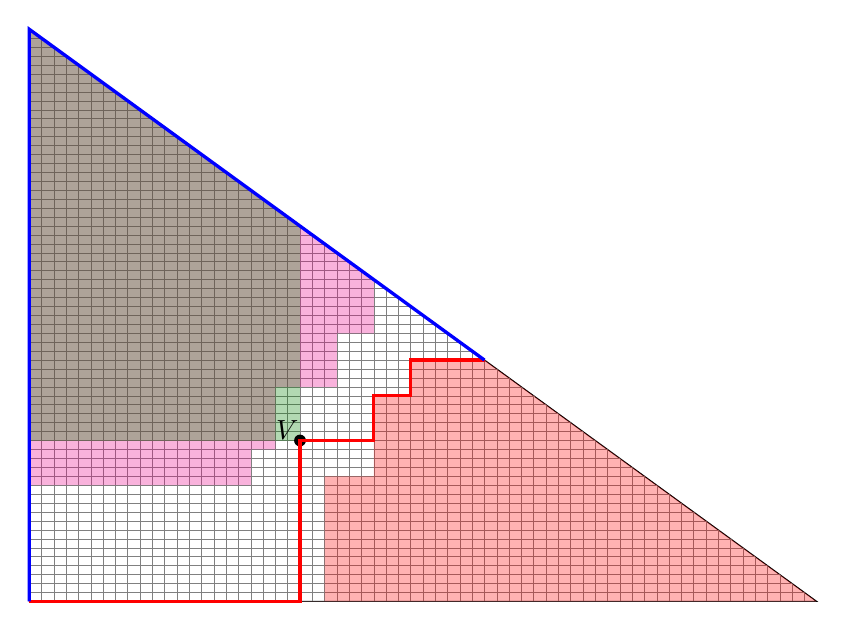
\begin{tikzpicture}[scale=10]
    \begin{scope}
    \draw[clip] (0,0.7265625) |- (1,0) --cycle;
    \draw[help lines,yscale=0.7265625] (0,0) grid[step=0.015625] (1,1);
    \fill[red,fill opacity=0.3] (0.0, 0.0)--(0.375, 0.0)--(0.375, 0.158935546875)--(0.4375, 0.158935546875)--(0.4375, 0.2611083984375)--(0.484375, 0.2611083984375)--(0.484375, 0.3065185546875)--(0.578125, 0.3065185546875)--(1, 0)--(0, 0) -- cycle;
\fill[magenta,fill opacity=0.3] (0.0, 0.0)--(0.0, 0.1475830078125)--(0.28125, 0.1475830078125)--(0.28125, 0.1929931640625)--(0.3125, 0.1929931640625)--(0.3125, 0.2724609375)--(0.390625, 0.2724609375)--(0.390625, 0.340576171875)--(0.4375, 0.340576171875)--(0.4375, 0.40869140625)--(0, 0.7265625) -- cycle;

    \fill[green!50!black,opacity=0.3] (0,0.7265625) rectangle (0.34375, 0.204345703125) node
    [shape=circle,fill=black,fill opacity=1,minimum size=1.5mm,inner sep=0pt,
    outer sep=0pt] {} node [above left=-3pt,black,opacity=1]
     { $V$};\end{scope}\draw[very thick, red](0.0, 0.0)--(0.34375, 0.0)--(0.34375, 0.204345703125)--(0.4375, 0.204345703125)--(0.4375, 0.2611083984375)--(0.484375, 0.2611083984375)--(0.484375, 0.3065185546875)--(0.578125, 0.3065185546875)coordinate (a);
\draw[very thick, blue] (a) -- (0,0.7265625) -- (0,0);
\end{tikzpicture}

\newpage
\item New vertex $p$ in lower excluded region $L^{5}$:
(26, 19) (in grid coordinates).

Vertices for the lower domain $D_L(p)$:

[(0, 13), (18, 13), (18, 17), (20, 17), (20, 18), (22, 18), (22, 19), (26, 19), (26, 30), (28, 30), (28, 36), [(64, 0), (0, 0)]]

Unprocessed eigenvalues for the lower domain:

[2.1682926349150446, 10.973311705699482]

Residuals:

[4.4606852769163212e-12, 6.9815231469825075e-12]

Rescaled eigenvalues (by bottom side length), but not postprocessed:

[ 12.32234011  62.36099167]

Postprocesses eigenvalue (lower bound):

12.3114070656

Eigenvalue for upper test domain $D_U^{test}$: 11.7853482551 (does not need to
be calculated until it reaches the threshold 12.25).

    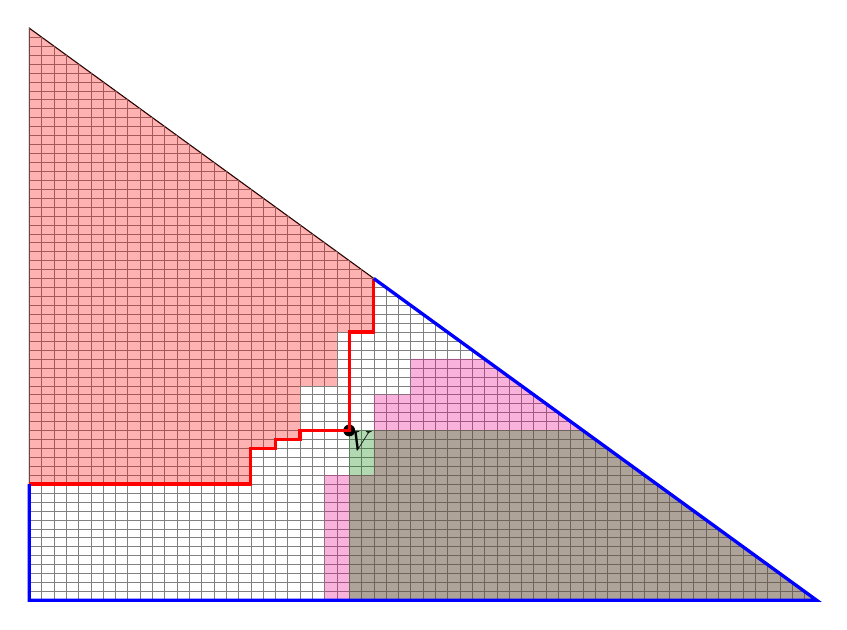
\begin{tikzpicture}[scale=10]
    \begin{scope}
    \draw[clip] (0,0.7265625) |- (1,0) --cycle;
    \draw[help lines,yscale=0.7265625] (0,0) grid[step=0.015625] (1,1);
    \fill[red,fill opacity=0.3] (0.0, 0.0)--(0.0, 0.1475830078125)--(0.28125, 0.1475830078125)--(0.28125, 0.1929931640625)--(0.3125, 0.1929931640625)--(0.3125, 0.204345703125)--(0.34375, 0.204345703125)--(0.34375, 0.2724609375)--(0.390625, 0.2724609375)--(0.390625, 0.340576171875)--(0.4375, 0.340576171875)--(0.4375, 0.40869140625)--(0, 0.7265625) -- cycle;
\fill[magenta,fill opacity=0.3] (0.0, 0.0)--(0.375, 0.0)--(0.375, 0.158935546875)--(0.4375, 0.158935546875)--(0.4375, 0.2611083984375)--(0.484375, 0.2611083984375)--(0.484375, 0.3065185546875)--(0.578125, 0.3065185546875)--(1, 0)--(0, 0) -- cycle;

    \fill[green!50!black,opacity=0.3] (1,0) rectangle (0.40625, 0.2156982421875) node
    [shape=circle,fill=black,fill opacity=1,minimum size=1.5mm,
    inner sep=0pt,outer sep=0pt] {} node [below right=-3pt,black,opacity=1]
     { $V$};\end{scope}\draw[very thick, red](0.0, 0.1475830078125)--(0.28125, 0.1475830078125)--(0.28125, 0.1929931640625)--(0.3125, 0.1929931640625)--(0.3125, 0.204345703125)--(0.34375, 0.204345703125)--(0.34375, 0.2156982421875)--(0.40625, 0.2156982421875)--(0.40625, 0.340576171875)--(0.4375, 0.340576171875)--(0.4375, 0.40869140625)coordinate (a);
\draw[very thick, blue] (a) -- (1,0) -- (0,0) -- (0.0, 0.1475830078125);
\end{tikzpicture}

\newpage
\item New vertex $p$ in upper excluded region $U^{6}$:
(28, 28) (in grid coordinates).

Vertices of the upper domain $D_U(p)$:

[(0, 0), (24, 0), (24, 14), (26, 14), (26, 19), (28, 19), (28, 28), (36, 28), [(0, 64)]]

Unprocessed eigenvalues for the upper domain:

[2.1591402221083222, 10.715800047494927]

Residuals:

[5.177504324617642e-12, 6.660217001865947e-12]

Rescaled eigenvalues (by the bottom side length), but not postprocessed:

[ 12.27032723  60.89756087]

Postprocesses eigenvalue (lower bound):

12.259486248

Eigenvalue for lower test domain $D_L^{test}$: 11.6697779075 (does not need to
be calculated until it reaches the threshold 12.25).

    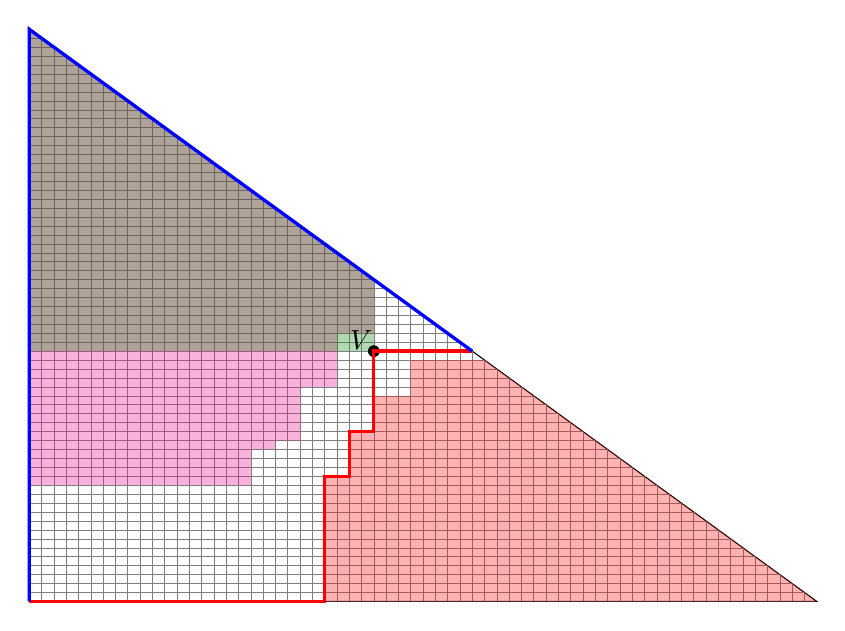
\begin{tikzpicture}[scale=10]
    \begin{scope}
    \draw[clip] (0,0.7265625) |- (1,0) --cycle;
    \draw[help lines,yscale=0.7265625] (0,0) grid[step=0.015625] (1,1);
    \fill[red,fill opacity=0.3] (0.0, 0.0)--(0.375, 0.0)--(0.375, 0.158935546875)--(0.40625, 0.158935546875)--(0.40625, 0.2156982421875)--(0.4375, 0.2156982421875)--(0.4375, 0.2611083984375)--(0.484375, 0.2611083984375)--(0.484375, 0.3065185546875)--(0.578125, 0.3065185546875)--(1, 0)--(0, 0) -- cycle;
\fill[magenta,fill opacity=0.3] (0.0, 0.0)--(0.0, 0.1475830078125)--(0.28125, 0.1475830078125)--(0.28125, 0.1929931640625)--(0.3125, 0.1929931640625)--(0.3125, 0.204345703125)--(0.34375, 0.204345703125)--(0.34375, 0.2724609375)--(0.390625, 0.2724609375)--(0.390625, 0.340576171875)--(0.4375, 0.340576171875)--(0.4375, 0.40869140625)--(0, 0.7265625) -- cycle;

    \fill[green!50!black,opacity=0.3] (0,0.7265625) rectangle (0.4375, 0.31787109375) node
    [shape=circle,fill=black,fill opacity=1,minimum size=1.5mm,inner sep=0pt,
    outer sep=0pt] {} node [above left=-3pt,black,opacity=1]
     { $V$};\end{scope}\draw[very thick, red](0.0, 0.0)--(0.375, 0.0)--(0.375, 0.158935546875)--(0.40625, 0.158935546875)--(0.40625, 0.2156982421875)--(0.4375, 0.2156982421875)--(0.4375, 0.31787109375)--(0.5625, 0.31787109375)coordinate (a);
\draw[very thick, blue] (a) -- (0,0.7265625) -- (0,0);
\end{tikzpicture}

\newpage
\item New vertex $p$ in lower excluded region $L^{6}$:
(21, 9) (in grid coordinates).

Vertices for the lower domain $D_L(p)$:

[(0, 9), (21, 9), (21, 18), (22, 18), (22, 24), (25, 24), (25, 28), (28, 28), (28, 36), [(64, 0), (0, 0)]]

Unprocessed eigenvalues for the lower domain:

[2.1648948969640949, 11.324730481768352]

Residuals:

[4.896413397690929e-12, 7.1156691027010294e-12]

Rescaled eigenvalues (by bottom side length), but not postprocessed:

[ 12.30303087  64.35809373]

Postprocesses eigenvalue (lower bound):

12.2921320482

Eigenvalue for upper test domain $D_U^{test}$: 11.8691352086 (does not need to
be calculated until it reaches the threshold 12.25).

    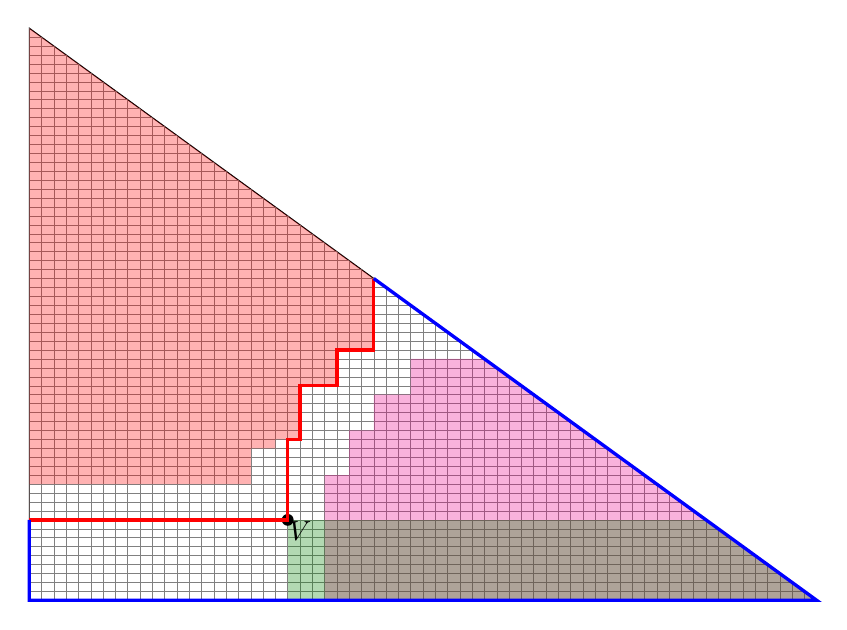
\begin{tikzpicture}[scale=10]
    \begin{scope}
    \draw[clip] (0,0.7265625) |- (1,0) --cycle;
    \draw[help lines,yscale=0.7265625] (0,0) grid[step=0.015625] (1,1);
    \fill[red,fill opacity=0.3] (0.0, 0.0)--(0.0, 0.1475830078125)--(0.28125, 0.1475830078125)--(0.28125, 0.1929931640625)--(0.3125, 0.1929931640625)--(0.3125, 0.204345703125)--(0.34375, 0.204345703125)--(0.34375, 0.2724609375)--(0.390625, 0.2724609375)--(0.390625, 0.31787109375)--(0.4375, 0.31787109375)--(0.4375, 0.40869140625)--(0, 0.7265625) -- cycle;
\fill[magenta,fill opacity=0.3] (0.0, 0.0)--(0.375, 0.0)--(0.375, 0.158935546875)--(0.40625, 0.158935546875)--(0.40625, 0.2156982421875)--(0.4375, 0.2156982421875)--(0.4375, 0.2611083984375)--(0.484375, 0.2611083984375)--(0.484375, 0.3065185546875)--(0.578125, 0.3065185546875)--(1, 0)--(0, 0) -- cycle;

    \fill[green!50!black,opacity=0.3] (1,0) rectangle (0.328125, 0.1021728515625) node
    [shape=circle,fill=black,fill opacity=1,minimum size=1.5mm,
    inner sep=0pt,outer sep=0pt] {} node [below right=-3pt,black,opacity=1]
     { $V$};\end{scope}\draw[very thick, red](0.0, 0.1021728515625)--(0.328125, 0.1021728515625)--(0.328125, 0.204345703125)--(0.34375, 0.204345703125)--(0.34375, 0.2724609375)--(0.390625, 0.2724609375)--(0.390625, 0.31787109375)--(0.4375, 0.31787109375)--(0.4375, 0.40869140625)coordinate (a);
\draw[very thick, blue] (a) -- (1,0) -- (0,0) -- (0.0, 0.1021728515625);
\end{tikzpicture}

\newpage
\item New vertex $p$ in upper excluded region $U^{7}$:
(29, 29) (in grid coordinates).

Vertices of the upper domain $D_U(p)$:

[(0, 0), (21, 0), (21, 9), (24, 9), (24, 14), (26, 14), (26, 19), (28, 19), (28, 23), (29, 23), (29, 29), (35, 29), [(0, 64)]]

Unprocessed eigenvalues for the upper domain:

[2.1588747785558096, 10.791541985379091]

Residuals:

[4.9585439614978746e-12, 6.8327913480466457e-12]

Rescaled eigenvalues (by the bottom side length), but not postprocessed:

[ 12.26881872  61.32799996]

Postprocesses eigenvalue (lower bound):

12.2579804048

Eigenvalue for lower test domain $D_L^{test}$: 11.805661388 (does not need to
be calculated until it reaches the threshold 12.25).

    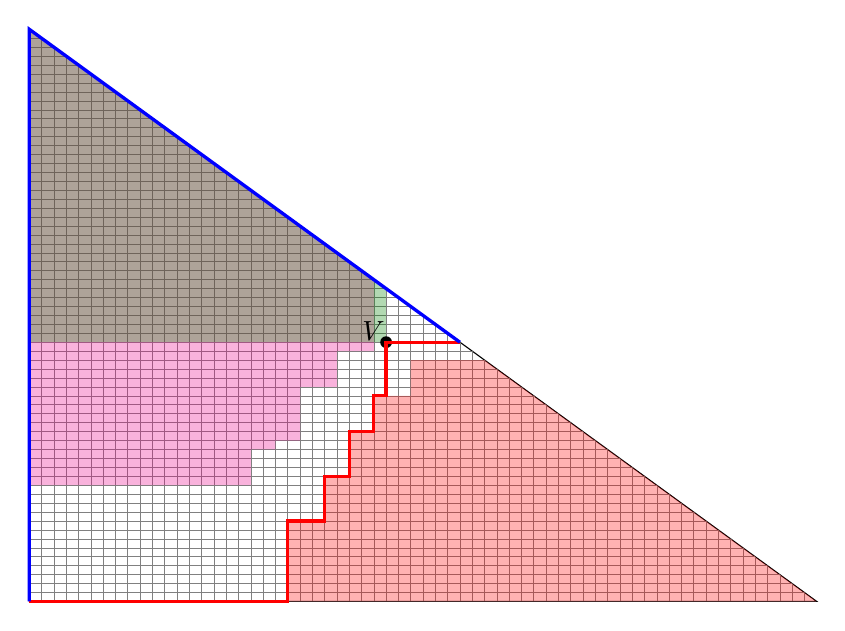
\begin{tikzpicture}[scale=10]
    \begin{scope}
    \draw[clip] (0,0.7265625) |- (1,0) --cycle;
    \draw[help lines,yscale=0.7265625] (0,0) grid[step=0.015625] (1,1);
    \fill[red,fill opacity=0.3] (0.0, 0.0)--(0.328125, 0.0)--(0.328125, 0.1021728515625)--(0.375, 0.1021728515625)--(0.375, 0.158935546875)--(0.40625, 0.158935546875)--(0.40625, 0.2156982421875)--(0.4375, 0.2156982421875)--(0.4375, 0.2611083984375)--(0.484375, 0.2611083984375)--(0.484375, 0.3065185546875)--(0.578125, 0.3065185546875)--(1, 0)--(0, 0) -- cycle;
\fill[magenta,fill opacity=0.3] (0.0, 0.0)--(0.0, 0.1475830078125)--(0.28125, 0.1475830078125)--(0.28125, 0.1929931640625)--(0.3125, 0.1929931640625)--(0.3125, 0.204345703125)--(0.34375, 0.204345703125)--(0.34375, 0.2724609375)--(0.390625, 0.2724609375)--(0.390625, 0.31787109375)--(0.4375, 0.31787109375)--(0.4375, 0.40869140625)--(0, 0.7265625) -- cycle;

    \fill[green!50!black,opacity=0.3] (0,0.7265625) rectangle (0.453125, 0.3292236328125) node
    [shape=circle,fill=black,fill opacity=1,minimum size=1.5mm,inner sep=0pt,
    outer sep=0pt] {} node [above left=-3pt,black,opacity=1]
     { $V$};\end{scope}\draw[very thick, red](0.0, 0.0)--(0.328125, 0.0)--(0.328125, 0.1021728515625)--(0.375, 0.1021728515625)--(0.375, 0.158935546875)--(0.40625, 0.158935546875)--(0.40625, 0.2156982421875)--(0.4375, 0.2156982421875)--(0.4375, 0.2611083984375)--(0.453125, 0.2611083984375)--(0.453125, 0.3292236328125)--(0.546875, 0.3292236328125)coordinate (a);
\draw[very thick, blue] (a) -- (0,0.7265625) -- (0,0);
\end{tikzpicture}

\newpage
\item New vertex $p$ in lower excluded region $L^{7}$:
(30, 27) (in grid coordinates).

Vertices for the lower domain $D_L(p)$:

[(0, 13), (18, 13), (18, 17), (20, 17), (20, 18), (22, 18), (22, 24), (25, 24), (25, 27), (30, 27), (30, 34), [(64, 0), (0, 0)]]

Unprocessed eigenvalues for the lower domain:

[2.1640230452714846, 10.759941376290984]

Residuals:

[4.4907304821988718e-12, 6.8071142541062353e-12]

Rescaled eigenvalues (by bottom side length), but not postprocessed:

[ 12.29807616  61.14841468]

Postprocesses eigenvalue (lower bound):

12.2871861146

Eigenvalue for upper test domain $D_U^{test}$: 11.94597256 (does not need to
be calculated until it reaches the threshold 12.25).

    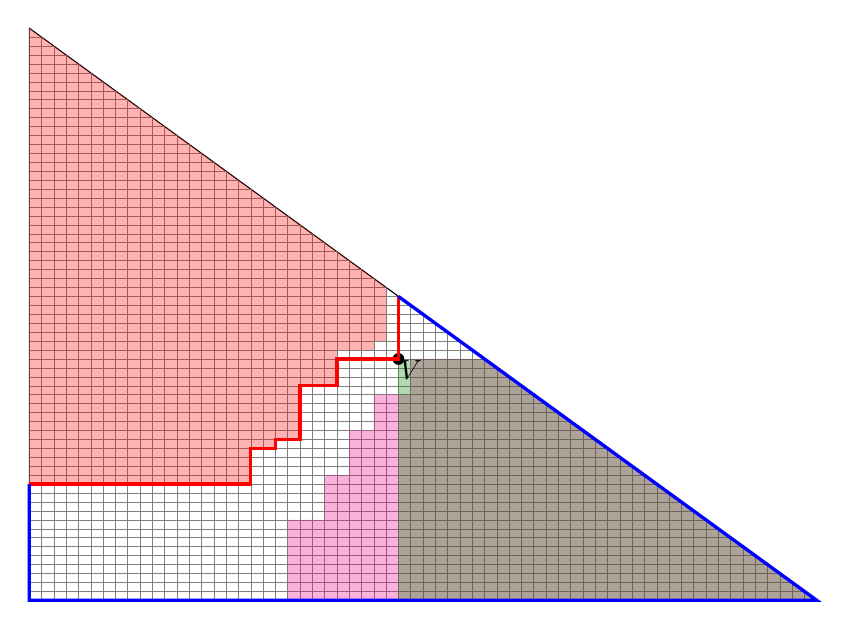
\begin{tikzpicture}[scale=10]
    \begin{scope}
    \draw[clip] (0,0.7265625) |- (1,0) --cycle;
    \draw[help lines,yscale=0.7265625] (0,0) grid[step=0.015625] (1,1);
    \fill[red,fill opacity=0.3] (0.0, 0.0)--(0.0, 0.1475830078125)--(0.28125, 0.1475830078125)--(0.28125, 0.1929931640625)--(0.3125, 0.1929931640625)--(0.3125, 0.204345703125)--(0.34375, 0.204345703125)--(0.34375, 0.2724609375)--(0.390625, 0.2724609375)--(0.390625, 0.31787109375)--(0.4375, 0.31787109375)--(0.4375, 0.3292236328125)--(0.453125, 0.3292236328125)--(0.453125, 0.3973388671875)--(0, 0.7265625) -- cycle;
\fill[magenta,fill opacity=0.3] (0.0, 0.0)--(0.328125, 0.0)--(0.328125, 0.1021728515625)--(0.375, 0.1021728515625)--(0.375, 0.158935546875)--(0.40625, 0.158935546875)--(0.40625, 0.2156982421875)--(0.4375, 0.2156982421875)--(0.4375, 0.2611083984375)--(0.484375, 0.2611083984375)--(0.484375, 0.3065185546875)--(0.578125, 0.3065185546875)--(1, 0)--(0, 0) -- cycle;

    \fill[green!50!black,opacity=0.3] (1,0) rectangle (0.46875, 0.3065185546875) node
    [shape=circle,fill=black,fill opacity=1,minimum size=1.5mm,
    inner sep=0pt,outer sep=0pt] {} node [below right=-3pt,black,opacity=1]
     { $V$};\end{scope}\draw[very thick, red](0.0, 0.1475830078125)--(0.28125, 0.1475830078125)--(0.28125, 0.1929931640625)--(0.3125, 0.1929931640625)--(0.3125, 0.204345703125)--(0.34375, 0.204345703125)--(0.34375, 0.2724609375)--(0.390625, 0.2724609375)--(0.390625, 0.3065185546875)--(0.46875, 0.3065185546875)--(0.46875, 0.385986328125)coordinate (a);
\draw[very thick, blue] (a) -- (1,0) -- (0,0) -- (0.0, 0.1475830078125);
\end{tikzpicture}

\newpage
\item New vertex $p$ in upper excluded region $U^{8}$:
(19, 12) (in grid coordinates).

Vertices of the upper domain $D_U(p)$:

[(0, 0), (19, 0), (19, 12), (24, 12), (24, 14), (26, 14), (26, 19), (28, 19), (28, 23), (30, 23), (30, 27), (37, 27), [(0, 64)]]

Unprocessed eigenvalues for the upper domain:

[2.1584009432958866, 11.023173768196036]

Residuals:

[5.0818345861509005e-12, 7.2845370544319738e-12]

Rescaled eigenvalues (by the bottom side length), but not postprocessed:

[ 12.26612593  62.64435623]

Postprocesses eigenvalue (lower bound):

12.2552923686

Eigenvalue for lower test domain $D_L^{test}$: 11.9274447895 (does not need to
be calculated until it reaches the threshold 12.25).

    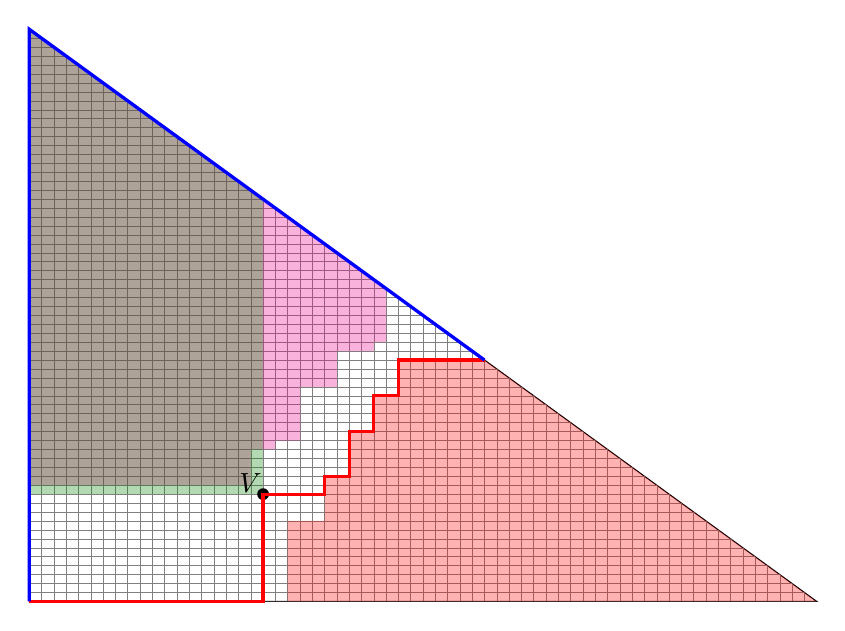
\begin{tikzpicture}[scale=10]
    \begin{scope}
    \draw[clip] (0,0.7265625) |- (1,0) --cycle;
    \draw[help lines,yscale=0.7265625] (0,0) grid[step=0.015625] (1,1);
    \fill[red,fill opacity=0.3] (0.0, 0.0)--(0.328125, 0.0)--(0.328125, 0.1021728515625)--(0.375, 0.1021728515625)--(0.375, 0.158935546875)--(0.40625, 0.158935546875)--(0.40625, 0.2156982421875)--(0.4375, 0.2156982421875)--(0.4375, 0.2611083984375)--(0.46875, 0.2611083984375)--(0.46875, 0.3065185546875)--(0.578125, 0.3065185546875)--(1, 0)--(0, 0) -- cycle;
\fill[magenta,fill opacity=0.3] (0.0, 0.0)--(0.0, 0.1475830078125)--(0.28125, 0.1475830078125)--(0.28125, 0.1929931640625)--(0.3125, 0.1929931640625)--(0.3125, 0.204345703125)--(0.34375, 0.204345703125)--(0.34375, 0.2724609375)--(0.390625, 0.2724609375)--(0.390625, 0.31787109375)--(0.4375, 0.31787109375)--(0.4375, 0.3292236328125)--(0.453125, 0.3292236328125)--(0.453125, 0.3973388671875)--(0, 0.7265625) -- cycle;

    \fill[green!50!black,opacity=0.3] (0,0.7265625) rectangle (0.296875, 0.13623046875) node
    [shape=circle,fill=black,fill opacity=1,minimum size=1.5mm,inner sep=0pt,
    outer sep=0pt] {} node [above left=-3pt,black,opacity=1]
     { $V$};\end{scope}\draw[very thick, red](0.0, 0.0)--(0.296875, 0.0)--(0.296875, 0.13623046875)--(0.375, 0.13623046875)--(0.375, 0.158935546875)--(0.40625, 0.158935546875)--(0.40625, 0.2156982421875)--(0.4375, 0.2156982421875)--(0.4375, 0.2611083984375)--(0.46875, 0.2611083984375)--(0.46875, 0.3065185546875)--(0.578125, 0.3065185546875)coordinate (a);
\draw[very thick, blue] (a) -- (0,0.7265625) -- (0,0);
\end{tikzpicture}

\newpage
\item New vertex $p$ in lower excluded region $L^{8}$:
(23, 15) (in grid coordinates).

Vertices for the lower domain $D_L(p)$:

[(0, 12), (19, 12), (19, 15), (23, 15), (23, 24), (25, 24), (25, 28), (28, 28), (28, 29), (29, 29), (29, 35), [(64, 0), (0, 0)]]

Unprocessed eigenvalues for the lower domain:

[2.1652787845040429, 11.133850073133729]

Residuals:

[4.4711438545278684e-12, 7.3874404717381035e-12]

Rescaled eigenvalues (by bottom side length), but not postprocessed:

[ 12.30521249  63.27332626]

Postprocesses eigenvalue (lower bound):

12.2943098053

Eigenvalue for upper test domain $D_U^{test}$: 12.0386343232 (does not need to
be calculated until it reaches the threshold 12.25).

    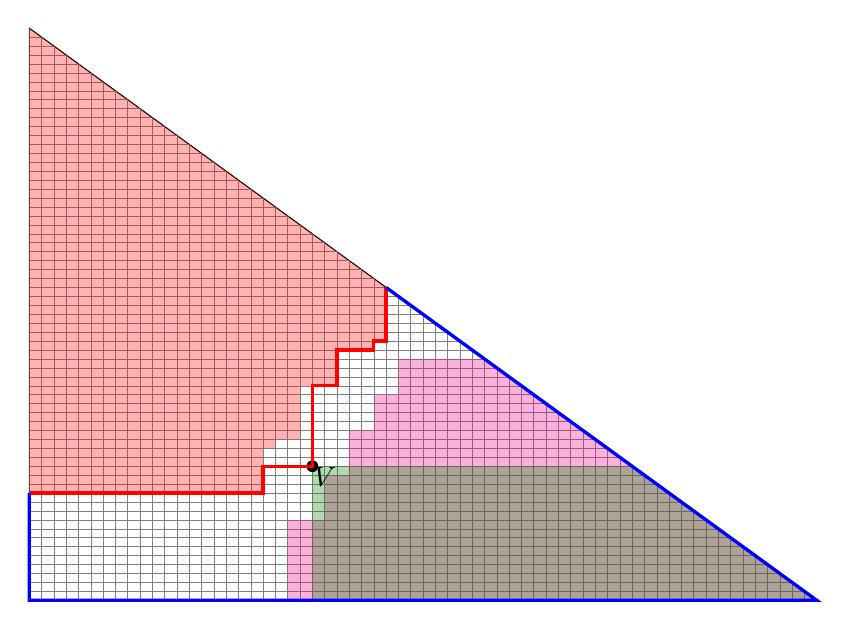
\begin{tikzpicture}[scale=10]
    \begin{scope}
    \draw[clip] (0,0.7265625) |- (1,0) --cycle;
    \draw[help lines,yscale=0.7265625] (0,0) grid[step=0.015625] (1,1);
    \fill[red,fill opacity=0.3] (0.0, 0.0)--(0.0, 0.13623046875)--(0.296875, 0.13623046875)--(0.296875, 0.1929931640625)--(0.3125, 0.1929931640625)--(0.3125, 0.204345703125)--(0.34375, 0.204345703125)--(0.34375, 0.2724609375)--(0.390625, 0.2724609375)--(0.390625, 0.31787109375)--(0.4375, 0.31787109375)--(0.4375, 0.3292236328125)--(0.453125, 0.3292236328125)--(0.453125, 0.3973388671875)--(0, 0.7265625) -- cycle;
\fill[magenta,fill opacity=0.3] (0.0, 0.0)--(0.328125, 0.0)--(0.328125, 0.1021728515625)--(0.375, 0.1021728515625)--(0.375, 0.158935546875)--(0.40625, 0.158935546875)--(0.40625, 0.2156982421875)--(0.4375, 0.2156982421875)--(0.4375, 0.2611083984375)--(0.46875, 0.2611083984375)--(0.46875, 0.3065185546875)--(0.578125, 0.3065185546875)--(1, 0)--(0, 0) -- cycle;

    \fill[green!50!black,opacity=0.3] (1,0) rectangle (0.359375, 0.1702880859375) node
    [shape=circle,fill=black,fill opacity=1,minimum size=1.5mm,
    inner sep=0pt,outer sep=0pt] {} node [below right=-3pt,black,opacity=1]
     { $V$};\end{scope}\draw[very thick, red](0.0, 0.13623046875)--(0.296875, 0.13623046875)--(0.296875, 0.1702880859375)--(0.359375, 0.1702880859375)--(0.359375, 0.2724609375)--(0.390625, 0.2724609375)--(0.390625, 0.31787109375)--(0.4375, 0.31787109375)--(0.4375, 0.3292236328125)--(0.453125, 0.3292236328125)--(0.453125, 0.3973388671875)coordinate (a);
\draw[very thick, blue] (a) -- (1,0) -- (0,0) -- (0.0, 0.13623046875);
\end{tikzpicture}

\newpage
\item New vertex $p$ in upper excluded region $U^{9}$:
(27, 25) (in grid coordinates).

Vertices of the upper domain $D_U(p)$:

[(0, 0), (21, 0), (21, 9), (23, 9), (23, 15), (26, 15), (26, 19), (27, 19), (27, 25), (30, 25), (30, 27), (37, 27), [(0, 64)]]

Unprocessed eigenvalues for the upper domain:

[2.1624388010101683, 10.864923641996144]

Residuals:

[4.9533761518189615e-12, 7.0740443674823618e-12]

Rescaled eigenvalues (by the bottom side length), but not postprocessed:

[ 12.28907295  61.74502565]

Postprocesses eigenvalue (lower bound):

12.2781988354

Eigenvalue for lower test domain $D_L^{test}$: 12.0541213255 (does not need to
be calculated until it reaches the threshold 12.25).

    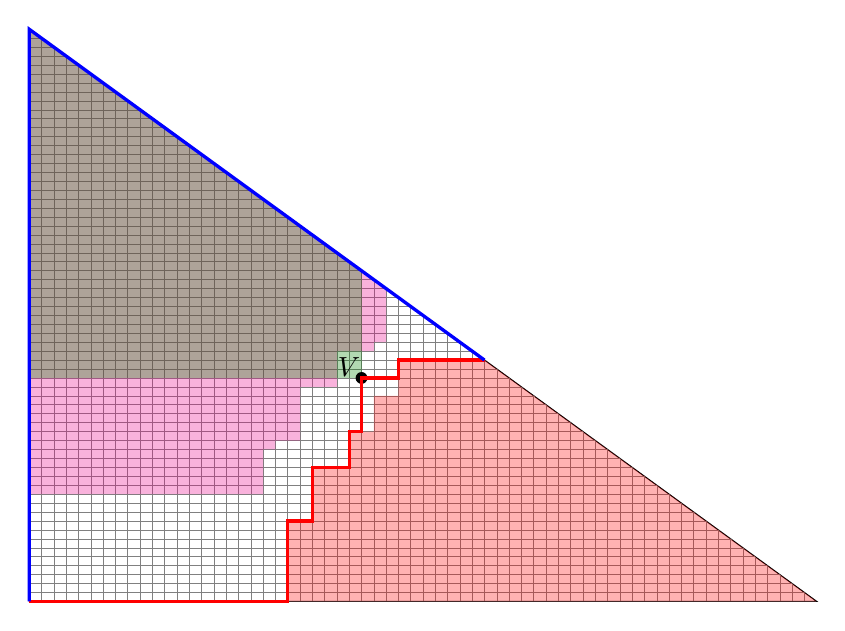
\begin{tikzpicture}[scale=10]
    \begin{scope}
    \draw[clip] (0,0.7265625) |- (1,0) --cycle;
    \draw[help lines,yscale=0.7265625] (0,0) grid[step=0.015625] (1,1);
    \fill[red,fill opacity=0.3] (0.0, 0.0)--(0.328125, 0.0)--(0.328125, 0.1021728515625)--(0.359375, 0.1021728515625)--(0.359375, 0.1702880859375)--(0.40625, 0.1702880859375)--(0.40625, 0.2156982421875)--(0.4375, 0.2156982421875)--(0.4375, 0.2611083984375)--(0.46875, 0.2611083984375)--(0.46875, 0.3065185546875)--(0.578125, 0.3065185546875)--(1, 0)--(0, 0) -- cycle;
\fill[magenta,fill opacity=0.3] (0.0, 0.0)--(0.0, 0.13623046875)--(0.296875, 0.13623046875)--(0.296875, 0.1929931640625)--(0.3125, 0.1929931640625)--(0.3125, 0.204345703125)--(0.34375, 0.204345703125)--(0.34375, 0.2724609375)--(0.390625, 0.2724609375)--(0.390625, 0.31787109375)--(0.4375, 0.31787109375)--(0.4375, 0.3292236328125)--(0.453125, 0.3292236328125)--(0.453125, 0.3973388671875)--(0, 0.7265625) -- cycle;

    \fill[green!50!black,opacity=0.3] (0,0.7265625) rectangle (0.421875, 0.2838134765625) node
    [shape=circle,fill=black,fill opacity=1,minimum size=1.5mm,inner sep=0pt,
    outer sep=0pt] {} node [above left=-3pt,black,opacity=1]
     { $V$};\end{scope}\draw[very thick, red](0.0, 0.0)--(0.328125, 0.0)--(0.328125, 0.1021728515625)--(0.359375, 0.1021728515625)--(0.359375, 0.1702880859375)--(0.40625, 0.1702880859375)--(0.40625, 0.2156982421875)--(0.421875, 0.2156982421875)--(0.421875, 0.2838134765625)--(0.46875, 0.2838134765625)--(0.46875, 0.3065185546875)--(0.578125, 0.3065185546875)coordinate (a);
\draw[very thick, blue] (a) -- (0,0.7265625) -- (0,0);
\end{tikzpicture}

\newpage
\item New vertex $p$ in lower excluded region $L^{9}$:
(31, 30) (in grid coordinates).

Vertices for the lower domain $D_L(p)$:

[(0, 12), (19, 12), (19, 17), (20, 17), (20, 18), (22, 18), (22, 24), (25, 24), (25, 25), (27, 25), (27, 28), (28, 28), (28, 29), (29, 29), (29, 30), (31, 30), (31, 33), [(64, 0), (0, 0)]]

Unprocessed eigenvalues for the lower domain:

[2.1640990008677603, 10.946325258072138]

Residuals:

[4.6336301266502685e-12, 7.8142078360388626e-12]

Rescaled eigenvalues (by bottom side length), but not postprocessed:

[ 12.29850781  62.20762852]

Postprocesses eigenvalue (lower bound):

12.2876170038

Eigenvalue for upper test domain $D_U^{test}$: 12.1584700213 (does not need to
be calculated until it reaches the threshold 12.25).

    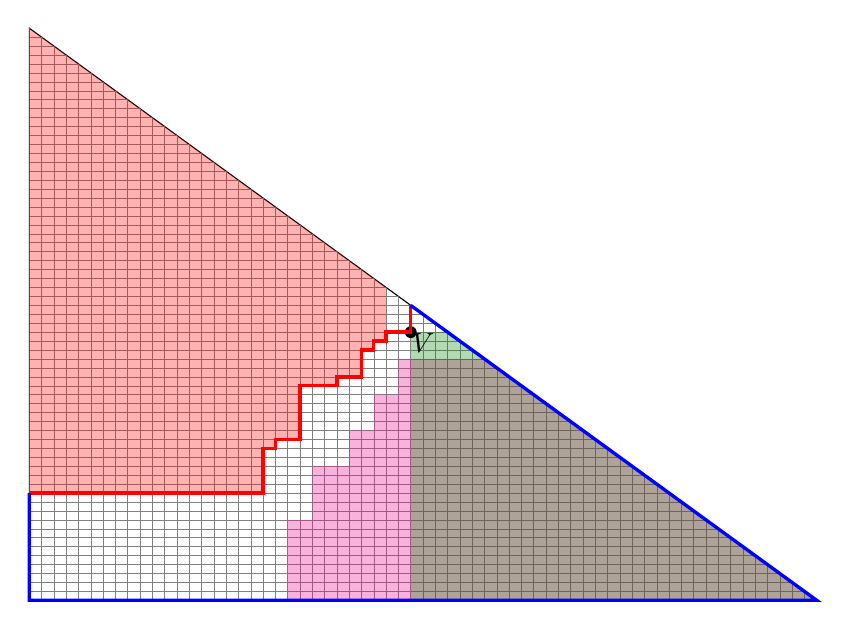
\begin{tikzpicture}[scale=10]
    \begin{scope}
    \draw[clip] (0,0.7265625) |- (1,0) --cycle;
    \draw[help lines,yscale=0.7265625] (0,0) grid[step=0.015625] (1,1);
    \fill[red,fill opacity=0.3] (0.0, 0.0)--(0.0, 0.13623046875)--(0.296875, 0.13623046875)--(0.296875, 0.1929931640625)--(0.3125, 0.1929931640625)--(0.3125, 0.204345703125)--(0.34375, 0.204345703125)--(0.34375, 0.2724609375)--(0.390625, 0.2724609375)--(0.390625, 0.2838134765625)--(0.421875, 0.2838134765625)--(0.421875, 0.31787109375)--(0.4375, 0.31787109375)--(0.4375, 0.3292236328125)--(0.453125, 0.3292236328125)--(0.453125, 0.3973388671875)--(0, 0.7265625) -- cycle;
\fill[magenta,fill opacity=0.3] (0.0, 0.0)--(0.328125, 0.0)--(0.328125, 0.1021728515625)--(0.359375, 0.1021728515625)--(0.359375, 0.1702880859375)--(0.40625, 0.1702880859375)--(0.40625, 0.2156982421875)--(0.4375, 0.2156982421875)--(0.4375, 0.2611083984375)--(0.46875, 0.2611083984375)--(0.46875, 0.3065185546875)--(0.578125, 0.3065185546875)--(1, 0)--(0, 0) -- cycle;

    \fill[green!50!black,opacity=0.3] (1,0) rectangle (0.484375, 0.340576171875) node
    [shape=circle,fill=black,fill opacity=1,minimum size=1.5mm,
    inner sep=0pt,outer sep=0pt] {} node [below right=-3pt,black,opacity=1]
     { $V$};\end{scope}\draw[very thick, red](0.0, 0.13623046875)--(0.296875, 0.13623046875)--(0.296875, 0.1929931640625)--(0.3125, 0.1929931640625)--(0.3125, 0.204345703125)--(0.34375, 0.204345703125)--(0.34375, 0.2724609375)--(0.390625, 0.2724609375)--(0.390625, 0.2838134765625)--(0.421875, 0.2838134765625)--(0.421875, 0.31787109375)--(0.4375, 0.31787109375)--(0.4375, 0.3292236328125)--(0.453125, 0.3292236328125)--(0.453125, 0.340576171875)--(0.484375, 0.340576171875)--(0.484375, 0.3746337890625)coordinate (a);
\draw[very thick, blue] (a) -- (1,0) -- (0,0) -- (0.0, 0.13623046875);
\end{tikzpicture}

\newpage
\item New vertex $p$ in upper excluded region $U^{10}$:
(25, 20) (in grid coordinates).

Vertices of the upper domain $D_U(p)$:

[(0, 0), (21, 0), (21, 9), (23, 9), (23, 15), (25, 15), (25, 20), (28, 20), (28, 23), (30, 23), (30, 27), (31, 27), (31, 30), (34, 30), [(0, 64)]]

Unprocessed eigenvalues for the upper domain:

[2.1612424885372805, 10.870469883392126]

Residuals:

[4.8441740893355694e-12, 6.7029987148089354e-12]

Rescaled eigenvalues (by the bottom side length), but not postprocessed:

[ 12.28227434  61.77654477]

Postprocesses eigenvalue (lower bound):

12.2714122515

Eigenvalue for lower test domain $D_L^{test}$: 12.2833697245 (does not need to
be calculated until it reaches the threshold 12.25).

    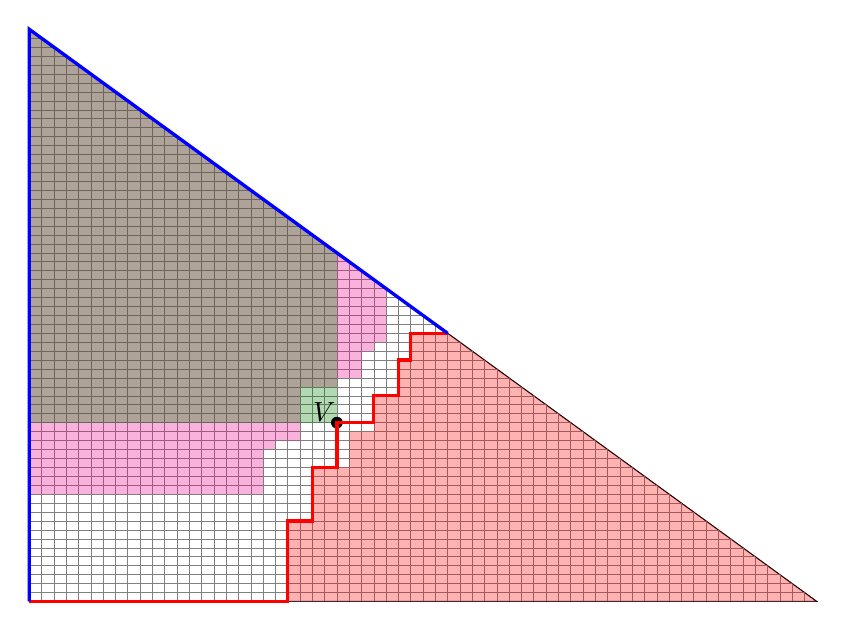
\begin{tikzpicture}[scale=10]
    \begin{scope}
    \draw[clip] (0,0.7265625) |- (1,0) --cycle;
    \draw[help lines,yscale=0.7265625] (0,0) grid[step=0.015625] (1,1);
    \fill[red,fill opacity=0.3] (0.0, 0.0)--(0.328125, 0.0)--(0.328125, 0.1021728515625)--(0.359375, 0.1021728515625)--(0.359375, 0.1702880859375)--(0.40625, 0.1702880859375)--(0.40625, 0.2156982421875)--(0.4375, 0.2156982421875)--(0.4375, 0.2611083984375)--(0.46875, 0.2611083984375)--(0.46875, 0.3065185546875)--(0.484375, 0.3065185546875)--(0.484375, 0.340576171875)--(0.53125, 0.340576171875)--(1, 0)--(0, 0) -- cycle;
\fill[magenta,fill opacity=0.3] (0.0, 0.0)--(0.0, 0.13623046875)--(0.296875, 0.13623046875)--(0.296875, 0.1929931640625)--(0.3125, 0.1929931640625)--(0.3125, 0.204345703125)--(0.34375, 0.204345703125)--(0.34375, 0.2724609375)--(0.390625, 0.2724609375)--(0.390625, 0.2838134765625)--(0.421875, 0.2838134765625)--(0.421875, 0.31787109375)--(0.4375, 0.31787109375)--(0.4375, 0.3292236328125)--(0.453125, 0.3292236328125)--(0.453125, 0.3973388671875)--(0, 0.7265625) -- cycle;

    \fill[green!50!black,opacity=0.3] (0,0.7265625) rectangle (0.390625, 0.22705078125) node
    [shape=circle,fill=black,fill opacity=1,minimum size=1.5mm,inner sep=0pt,
    outer sep=0pt] {} node [above left=-3pt,black,opacity=1]
     { $V$};\end{scope}\draw[very thick, red](0.0, 0.0)--(0.328125, 0.0)--(0.328125, 0.1021728515625)--(0.359375, 0.1021728515625)--(0.359375, 0.1702880859375)--(0.390625, 0.1702880859375)--(0.390625, 0.22705078125)--(0.4375, 0.22705078125)--(0.4375, 0.2611083984375)--(0.46875, 0.2611083984375)--(0.46875, 0.3065185546875)--(0.484375, 0.3065185546875)--(0.484375, 0.340576171875)--(0.53125, 0.340576171875)coordinate (a);
\draw[very thick, blue] (a) -- (0,0.7265625) -- (0,0);
\end{tikzpicture}

\end{enumerate}
\end{document}